%! Author = Kevin Lin
%! Date = 10/22/2026

% Preamble
\documentclass[11pt,a4paper,margin=1in]{article}

% Packages
\usepackage{amsmath}
\usepackage{amssymb}
\usepackage{enumerate}
\usepackage{pdfpages}

\title{HW 4}
\author{Kevin Lin}
\date{10/22/2026}

% Document
\begin{document}
\maketitle

\section{}
\begin{enumerate}[(a)]
    \item By the cone condition (0.1) $\|\Delta_{S^c}\|_1 \leq 3\|\Delta_S\|_1$.
    Since $S$ and $S^c$ partition the coordinates of $\Delta$, we have:
    \begin{align*}
        \|\Delta\|_1 &= \|\Delta_S\|_1 + \|\Delta_{S^c}\|_1 \\
        &\leq \|\Delta_S\|_1 + 3\|\Delta_S\|_1 \\
        &= 4\|\Delta_S\|_1
    \end{align*}
    Because $|S| = k$, applying the Cauchy-Schwarz inequality gives:
    \begin{align*}
        \|\Delta_S\|_1 &\leq \sum_{i \in S} |\Delta_i| \\
        &\leq \sqrt{k}\sqrt{\sum_{i \in S} |\Delta_i|^2} \\
        &= \sqrt{k}\|\Delta_S\|_2
    \end{align*}
    Combining the two inequalities gives us $\|\Delta\|_1 \leq 4\sqrt{k}\|\Delta_S\|_2$.
    Substituting the $\ell_2$ bound (0.2) gives us:
    \begin{align*}
        \|\Delta\|_1 &\leq 4\sqrt{k}\left(\frac{3\lambda\sqrt{k}}{\kappa}\right) \\
        &= \frac{12\lambda k}{\kappa}
    \end{align*}
    Thus, $\|\Delta\|_1 \leq \frac{12\lambda k}{\kappa}$.
    \item For any $q \in [1,2]$, we can define the Holder conjugates $a = \frac{1}{2 - q}$
    and $b = \frac{1}{q - 1}$ such that $\frac{1}{a} + \frac{1}{b} = 1$. By the
    definition of the $\ell_q$ norm, we have $\|v\|_q^q = \sum_{i=1}^p |v_i|^q$.
    We can rewrite each term $|v_i|^q = |v_i|^{2-q}|v_i|^{2(q-1)}$ and apply 
    Holder's inequality to get:
    \begin{align*}
        \sum_{i=1}^p |v_i|^q &= \sum_{i=1}^p |v_i|^{2-q}|v_i|^{2(q-1)} \\
        &\leq \left(\sum_{i=1}^p |v_i|^{(2-q)a}\right)^{\frac{1}{a}}\left(\sum_{i=1}^p |v_i|^{2(q-1)b}\right)^{\frac{1}{b}} \\
        \|v\|_q^q &= \left(\sum_{i=1}^p |v_i|\right)^{2-q}\left(\sum_{i=1}^p |v_i|^2\right)^{q-1} \\
        &= \|v\|_1^{2-q}\|v\|_2^{2(q-1)} \\
        \|v\|_q &\leq \|v\|_1^{\frac{2-q}{q}}\|v\|_2^{\frac{2(q-1)}{q}} \\
        &= \|v\|_1^{2/q - 1}\|v\|_2^{2 - 2/q}
    \end{align*}
    For $q = 1, 2$, the inequality holds with equality, thus $\|v\|_q \leq \|v\|_1^{2/q - 1}\|v\|_2^{2 - 2/q}$ 
    for all $q \in [1,2]$. Using the bounds from (a) and (0.2), $\|\Delta\|_1 \leq \frac{12\lambda k}{\kappa}$
    and $\|\Delta\|_2 \leq \frac{3\lambda\sqrt{k}}{\kappa}$. We can substitue these
    bounds into the inequality to get:
    \begin{align*}
        \|\Delta\|_q &\leq \left(\frac{12\lambda k}{\kappa}\right)^{2/q - 1}\left(\frac{3\lambda\sqrt{k}}{\kappa}\right)^{2 - 2/q} \\
        &= \left(\frac{\lambda}{\kappa}\right)^{\frac{2}{q} - 1 + 2 - \frac{2}{q}} \cdot k^{\frac{2}{q} - 1 + \frac{2 - 2/q}{2}} \cdot 12^{\frac{2}{q} - 1} \cdot 3^{2 - \frac{2}{q}} \\
        &= \left(\frac{\lambda}{\kappa}\right) \cdot k^{1/q} \cdot 4^{2/q - 1} \cdot 3 \\
        &= 3 \cdot 4^{2/q - 1} \frac{k^{1/q}\lambda}{\kappa}
    \end{align*}
    For $q = 1$, the constant is $3 \cdot 4^{2 - 1} = 12$, and for $q = 2$, the 
    constant is $3 \cdot 4^{1 - 1} = 3$, so both are always $\leq 12$. Thus, we 
    have $\|\Delta\|_q \leq \frac{12k^{1/q}\lambda}{\kappa}$ for all $q \in [1,2]$.
    When $q = 1$, we have $\|\Delta\|_1 \leq \frac{12k\lambda}{\kappa}$ which
    recovers (a), and when $q = 2$, we have $\|\Delta\|_2 \leq \frac{3\sqrt{k}\lambda}{\kappa}$
    which recovers (0.2).
    \item Utilize (0.1) $\frac{1}{2n}\|X\Delta\|_2^2 \leq \frac{3\lambda}{2}\|\Delta_S\|_1 - \frac{\lambda}{2}\|\Delta_{S^c}\|_1$.
    Because $\|Delta_{S^c}\|_1 \geq 0$, we can drop the second term on the right-hand side to get:
    \begin{align*}
        \frac{1}{2n}\|X\Delta\|_2^2 &\leq \frac{3\lambda}{2}\|\Delta_S\|_1 \\
        \frac{1}{n}\|X\Delta\|_2^2 &\leq 3\lambda\|\Delta_S\|_1
    \end{align*}
    By Cauchy-Schwarz, since $|S| = k$, $\|Delta_S\|_1 \leq \sqrt{k}\|\Delta_S\|_2 \leq \sqrt{k}\|\Delta\|_2$. 
    Substituting this into the inequality gives $\frac{1}{n}\|X\Delta\|_2^2 \leq 3\lambda\sqrt{k}\|\Delta\|_2$.
    We can then apply the $\ell_2$ bound (0.2) to get:
    \begin{align*}
        \frac{1}{n}\|X\Delta\|_2^2 &\leq 3\lambda\sqrt{k}\left(\frac{3\lambda\sqrt{k}}{\kappa}\right) \\
        &= \frac{9k\lambda^2}{\kappa}
    \end{align*}
    Thus, $\frac{1}{n}\|X\Delta\|_2^2 \leq \frac{9k\lambda^2}{\kappa}$.
    \item With the assumptions, by the optimality of the LASSO estimator, the objective 
    value is no larger than the objective value $\beta^*$:
    \[
        \frac{1}{2n}\|y - X\hat{\beta}\|_2^2 + \lambda\|\hat{\beta}\|_1 \leq \frac{1}{2n}\|y - X\beta^*\|_2^2 + \lambda\|\beta^*\|_1 \\
    \]
    We know that $y = X\beta^* + \epsilon$, $\hat{\beta} = \beta^* + \Delta$, thus
    $y - X\hat{\beta} = \epsilon - X\Delta$ and $y - X\beta^* = \epsilon$. Substituting 
    these into the inequality gives:
    \begin{align*}
        \frac{1}{2n}\|\epsilon - X\Delta\|_2^2 + \lambda\|\beta^* + \Delta\|_1 &\leq \frac{1}{2n}\|\epsilon\|_2^2 + \lambda\|\beta^*\|_1 \\
        \|\epsilon - X\Delta\|_2^2 &= \|\epsilon\|_2^2 - 2\epsilon^\top X\Delta + \|X\Delta\|_2^2 \\
        \frac{1}{2n}\|X\Delta\|_2^2 + \lambda\|\hat{\beta}\|_1 &\leq \frac{1}{n}\epsilon^\top X\Delta + \lambda\|\beta^*\|_1
    \end{align*}
    Using Holder's inequality and the noise condition:
    \begin{align*}
        \frac{1}{n}\epsilon^TX\Delta &\leq \left(\frac{1}{n}X^\top\epsilon\right)^\top\Delta \\
        &\leq \|\frac{1}{n}X^\top\epsilon\|_\infty\|\Delta\|_1 \\
        &\leq \frac{\lambda}{2}\|\Delta\|_1
    \end{align*}
    Thus, $\frac{1}{2n}\|X\Delta\|_2^2 + \lambda\|\hat{\beta}\|_1 \leq \frac{\lambda}{2}\|\Delta\|_1 + \lambda\|\beta^*\|_1$.
    By the triangle inequality, $\|\Delta\|_1 = \|\hat{\beta} - \beta^*\|_1 \leq \|\hat{\beta}\|_1 + \|\beta^*\|_1$, 
    so we can substitute this into the inequality to get:
    \begin{align*}
        \frac{1}{2n}\|X\Delta\|_2^2 + \lambda\|\hat{\beta}\|_1 &\leq \frac{\lambda}{2}(\|\hat{\beta}\|_1 + \|\beta^*\|_1) + \lambda\|\beta^*\|_1 \\
        &= \frac{\lambda}{2}\|\hat{\beta}\|_1 + \frac{3\lambda}{2}\|\beta^*\|_1 \\
        \frac{1}{2n}\|X\Delta\|_2^2 + \frac{\lambda}{2}\|\hat{\beta}\|_1 &\leq \frac{3\lambda}{2}\|\beta^*\|_1 \\
        \frac{1}{n}\|X\Delta\|_2^2 + \lambda\|\hat{\beta}\|_1 &\leq 3\lambda\|\beta^*\|_1
    \end{align*}
    Because $\lambda\|\hat{\beta}\|_1 \geq 0$, we can drop this term to get $\frac{1}{n}\|X\Delta\|_2^2 \leq 3\lambda\|\beta^*\|_1$.
    Because the prediction error is nonnegative, $\frac{1}{n}\|X\Delta\|_2^2 \geq 0$, 
    we can drop this term to get $\lambda\|\hat{\beta}\|_1 \leq 3\lambda\|\beta^*\|_1$.
    We know $\lambda > 0$, so we can get $\|\hat{\beta}\|_1 \leq 3\|\beta^*\|_1$.

    Now, taking $\lambda \asymp \sigma\sqrt{\frac{\log p}{n}}$ and assuming $\beta^*$
    has $k$ nonzero entries, each equal to $\pm1$, $\|\beta^*\|_1 = \sum{i=1}^p |\beta^*_i| = k$. 
    Then the fast rate from (c):
    \begin{align*}
        \frac{1}{n}\|X\Delta\|_2^2 &\leq \frac{9k\lambda^2}{\kappa} \\
        &\lesssim \frac{9k\sigma^2\log p}{\kappa n} 
    \end{align*}
    For fixed $k, p, \sigma, \kappa$, this is $\mathcal{O}(1/n)$. \\
    The slow rate from (d):
    \begin{align*}
            \frac{1}{n}\|X\Delta\|_2^2 &\leq 3\lambda\|\beta^*\|_1 = 3k\lambda\\
            &\lesssim 3k\sigma\sqrt{\frac{\log p}{n}}
    \end{align*}
    For fixed $k, p, \sigma$, this is $\mathcal{O}(1/\sqrt{n})$. \\
    Comparing the bounds:
    \begin{align*}
        \frac{9k\lambda^2}{\kappa} &\leq 3k\lambda \\
        \frac{3\lambda}{\kappa} &\leq 1 \\
        \lambda &\leq \frac{\kappa}{3}
    \end{align*}
    We know $\lambda \asymp \sigma\sqrt{\frac{\log p}{n}}$, so $\sigma\sqrt{\frac{\log p}{n}} \leq \frac{\kappa}{3}$.
    Rearrange for $n$ gives $n \geq \frac{9\sigma^2\log p}{\kappa^2}$. Thus, the fast rate 
    is better than the slow rate when $n \gtrsim \frac{9\sigma^2\log p}{\kappa^2}$.
\end{enumerate}

\section{}
\begin{enumerate}[(a)]
    \item Let $u \in \mathbb{R}^p$ such that $\|u\|_2 = 1$, $\|u\|_0 \leq k$. 
    Let $T = \text{supp}(u)$, then $|T| \leq k$. Then, by the triangle
    inequality and definitions of $\delta_1(A)$ and $\mu(A)$:
    \begin{align*}
        \|Au\|_2^2 - 1 &= u^\top (A^\top A - I)u \\
        &= \sum_{j \in T} u_j^2(\|A_j\|_2^2 - 1) + \sum_{i,j \in T, i \neq j} u_iu_j A_i^\top A_j \\
        &\leq \delta_1(A)\sum_{j \in T} u_j^2 + \mu(A)\sum_{i,j \in T, i \neq j} |u_i||u_j| \\
        &= \delta_1(A) + \mu(A)\left[\left(\sum_{j \in T} |u_j|\right)^2 - \sum_{j \in T} u_j^2\right] \\
        &= \delta_1(A) + \mu(A)\left[\|u\|_1^2 - 1\right] \\
    \end{align*}
    Since $u$ has at most $k$ nonzero coordinates, by Cauchy-Schwarz, 
    $\|u\|_1 \leq \sqrt{k}\|u\|_2 = \sqrt{k}$. Therefore, $\|u\|_1^2 - 1 \leq k - 1$,
    and we have $|\|Au\|_2^2 - 1| \leq \delta_1(A) + (k - 1)\mu(A)$. Taking 
    the supremum over every $k$-sparse unit vector $u$ gives us
    $\delta_k(A) \leq \delta_1(A) + (k - 1)\mu(A)$.
    \item We start by bounding $\delta_1(A)$. For every column $j$, $\|A_j\|_2^2 - 1 = \frac{1}{n}\sum_{i=1}^n(X_{ij}^2 - 1)$. 
    Since $X_{ij} \sim \mathcal{N}(0,1)$, $E[X_{ij}^2 - 1] = 0$, and the centered
    squares are sub-exponential. If we apply Bernstein's inequality, there then
    exists an absolute constant $c > 0$ such that:
    \[
        P(|\|A_j\|_2^2 - 1| \geq t) \leq 2\exp(-cnt^2) \quad \forall 0 < t \leq 1
    \]
    Applying the union bound over all $p$ columns gives:
    \begin{align*}
        P(\delta_1(A) \geq t) &= P\left(\max_{j=1,\ldots,p}|\|A_j\|_2^2 - 1| \geq t\right) \\
        &\leq \sum_{j=1}^p P(|\|A_j\|_2^2 - 1| \geq t) \\
        &\leq 2p\exp(-cnt^2)
    \end{align*}
    Now we bound $\mu(A)$. For distinct columns $i \neq j$, $A_i^\top A_j = \frac{1}{n}\sum_{k=1}^n X_{ki}X_{kj}$.
    Because each entry is independent and nonzero, $E[X_{ki}X_{kj}] = 0$, and the 
    product of independent Gaussians is sub-exponential. Thus, again with Bernstein's
    inequality, we have $P(|A_i^\top A_j| \geq t) \leq 2\exp(-cnt^2)$ for some 
    absolute constant $c > 0$ and $0 < t \leq 1$. There are $\binom{p}{2}$ distinct
    pairs of columns, thus applying the union bound gives:
    \begin{align*}
        P(\mu(A) \geq t) &= P\left(\max_{i,j=1,\ldots,p, i \neq j}|A_i^\top A_j| \geq t\right) \\
        &\leq \sum_{i,j=1,\ldots,p, i \neq j} P(|A_i^\top A_j| \geq t) \\
        &\leq 2\binom{p}{2}\exp(-cnt^2) \\
        &\leq p^2\exp(-cnt^2)
    \end{align*}
    Now we combine the two bounds:
    \begin{align*}
        P(\delta_1(A) \geq t \text{ or } \mu(A) \geq t) &\leq 2p\exp(-cnt^2) + p^2\exp(-cnt^2) \\
        &\leq 2p^2\exp(-cnt^2), \quad p \geq 2 
    \end{align*}
    Choose $t = C\sqrt{\frac{\log p}{n}}$ with $C = \sqrt{3/c}$. Then $cnt^2 = 3\log p$, and we have:
    \begin{align*}
        P(\delta_1(A) \geq C\sqrt{\frac{\log p}{n}} \text{ or } \mu(A) \geq C\sqrt{\frac{\log p}{n}}) &\leq 2p^2\exp(-3\log p) \\
        &= 2p^2p^{-3} = 2/p
    \end{align*}
    For $n \geq C'\log p$, with $C' \geq C^2$, we have $t \leq 1$, and thus with
    probability at least $1 - 2/p$, $\delta_1(A) \leq C\sqrt{\frac{\log p}{n}}$ and
    $\mu(A) \leq C\sqrt{\frac{\log p}{n}}$.
    \item From (a), we have $\delta_k(A) \leq \delta_1(A) + (k - 1)\mu(A)$. From (b), 
    with probability at least $1 - 2/p$, $\delta_1(A) \leq C\sqrt{\frac{\log p}{n}}$ and
    $\mu(A) \leq C\sqrt{\frac{\log p}{n}}$. Thus, with probability at least $1 - 2/p$:
    \begin{align*}
        \delta_k(A) &\leq C\sqrt{\frac{\log p}{n}} + (k - 1)C\sqrt{\frac{\log p}{n}} \\
        &= kC\sqrt{\frac{\log p}{n}}
    \end{align*}
    To guarantee $k$-RIP with constant $\delta$, we require $kC\sqrt{\frac{\log p}{n}} \leq \delta$, 
    which rearranges to $n \geq C^2\delta^{-2}k^2\log p$. Taking $C'' = C^2$, or
    a larger absolute constant as necessary, gives $n \geq C''\delta^{-2}k^2\log p$.
    Thus, for $0 < \delta < 1$, this sample size guarantees $k$-RIP with probability
    at least $1 - 2/p$. \\
    $k$ is lost in (a) when we bound all off diagonal entires using the worst
    case coherence: $\sum_{i \neq j} |u_i||u_j||\left<A_i, A_j\right>| \leq (k - 1)\mu(A)$.
    Since $\mu(A) \lesssim \sqrt{\frac{\log p}{n}}$, we need to multiply by $k$ 
    to account for the $k$ nonzero entries in $u$. This is a loose bound because
    taking the absolute value ignores cancellation among the off diagonal entries, 
    and thus we get $\delta_k(A) \lesssim k\sqrt{\frac{\log p}{n}}$. Squaring the
    resulting sample size condition introduces the $k^2$ term. \\
    For a fixed $k$-sparse unit vector $u$, Bernstein's inequality gives:
    \[
        P(|\|Au\|_2^2 - 1| \geq \delta) \leq 2\exp(-cn\delta^2)
    \]
    for $0 < \delta < 1$. A $1/4$-net for the $k$-spare unit sphere has size
    at most $|\mathcal{N}| \leq 9^k\binom{p}{k} \leq \left(\frac{9ep}{k}\right)^k$. 
    Applying the union bound and the net-to-sphere argument after adjusting 
    absolute constants gives $P(\delta_k(A) \geq \delta) \leq 2\exp\left(-cn\delta^2 + k\log(9ep/k)\right)$.
    Thus, $k$-RIP holds with high probability when $n \gtrsim \delta^{-2}k\log(ep/k)$.
    Unlike the coherence argument, the net argument controls all sparse directions
    instead of summing over the worst case coherence, and thus avoids the loose $k$ factor.
\end{enumerate}

\section{}
\begin{enumerate}[(a)]
    \item The matrix exponential of a square matrix $A$ is defined by the
    convergent power series $e^A = \sum_{n=0}^{\infty} \frac{A^n}{n!}$. Therefore,
    $e^{X + Y} = \sum_{n=0}^{\infty} \frac{(X + Y)^n}{n!}$. Since $XY = YX$, we
    can apply the binomial theorem $(X + Y)^n = \sum_{k=0}^{n} \binom{n}{k} X^k Y^{n-k}$. 
    Substituting this into the exponential series gives:
    \begin{align*}
        e^{X + Y} &= \sum_{n=0}^{\infty} \frac{(X + Y)^n}{n!} \\
        &= \sum_{n=0}^{\infty} \frac{1}{n!} \sum_{k=0}^{n} \binom{n}{k} X^k Y^{n-k} \\
        &= \sum_{n=0}^{\infty} \sum_{k=0}^{n} \frac{X^k Y^{n-k}}{k! (n-k)!}
    \end{align*}
    Let $m = n - k$. Since $k, m \geq 0$, we can rearrange the absolutely convergent
    series:
    \begin{align*}
        e^{X + Y} &= \sum_{k=0}^{\infty} \sum_{m=0}^{\infty} \frac{X^k Y^m}{k! m!} \\
        &= \left(\sum_{k=0}^{\infty} \frac{X^k}{k!}\right) \left(\sum_{m=0}^{\infty} \frac{Y^m}{m!}\right) \\
        &= e^X e^Y
    \end{align*}
    Thus, for commuting matrices $X$ and $Y$, we have $e^{X + Y} = e^X e^Y$.
    \item Consider the symmetric matrices:
    \[
        X = \begin{bmatrix}
            1 & 0 \\
            0 & 0
        \end{bmatrix}, \quad
        Y = \begin{bmatrix}
            0 & 1 \\
            1 & 0   
        \end{bmatrix}
    \]
    Since $X$ is diagonal, its matrix exponential is $e^X = \begin{bmatrix}
        e & 0 \\
        0 & 1
    \end{bmatrix}$. Note that $Y^2 = I$, so $Y^{2m} = I$ and $Y^{2m+1} = Y$. Therefore,
    using the matrix exponential series, we get:
    \begin{align*}
        e^Y &= \sum_{m = 0}^\infty \frac{Y^m}{m!} \\
        &= \sum_{m = 0}^\infty \frac{Y^{2m}}{(2m)!} + \sum_{m = 0}^\infty \frac{Y^{2m+1}}{(2m+1)!} \\
        &= \sum_{m = 0}^\infty \frac{I}{(2m)!} + \sum_{m = 0}^\infty \frac{Y}{(2m+1)!} \\
        &= \left(\sum_{m = 0}^\infty \frac{1}{(2m)!}\right) I + \left(\sum_{m = 0}^\infty \frac{1}{(2m+1)!}\right) Y \\
        &= \cosh(1) I + \sinh(1) Y \\
        &= \begin{bmatrix}
            \cosh(1) & \sinh(1) \\
            \sinh(1) & \cosh(1)
        \end{bmatrix}
    \end{align*}
    Therefore, 
    \begin{align*}
        e^Xe^Y &= \begin{bmatrix}
            e & 0 \\
            0 & 1
        \end{bmatrix} \begin{bmatrix}
            \cosh(1) & \sinh(1) \\
            \sinh(1) & \cosh(1)
        \end{bmatrix} \\
        &= \begin{bmatrix}
            e\cosh(1) & e\sinh(1) \\
            \sinh(1) & \cosh(1)
        \end{bmatrix}
    \end{align*}
    Note that this matrix is not symmetric since $e\sinh(1) \neq \sinh(1)$. However,
    $X + Y$ is symmetric, and the exponential of a symmetric matrix is also symmetric
    because $(e^{X + Y})^\top = e^{(X + Y)^\top} = e^{X + Y}$. Thus, $e^{X + Y}$ 
    is symmetric while $e^Xe^Y$ is not, therefore they can't be equal.
\end{enumerate}

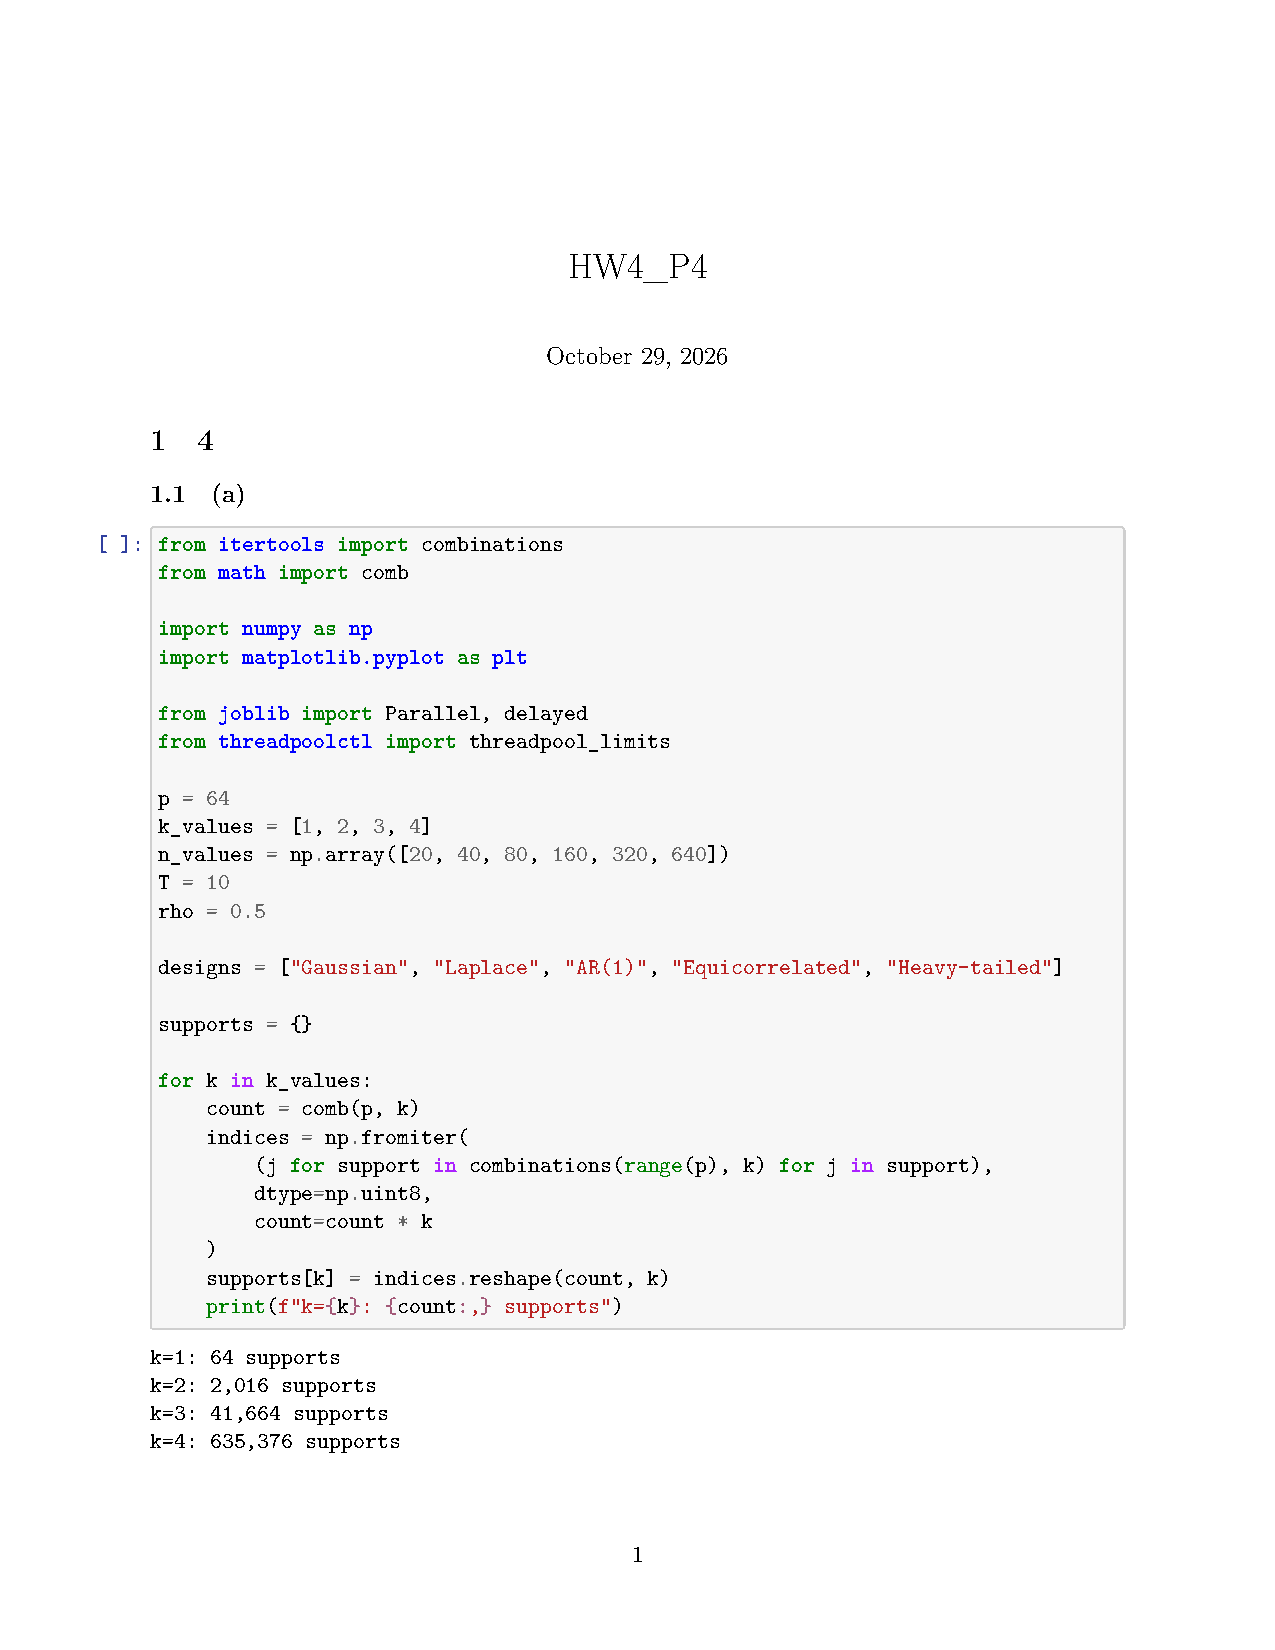
\includepdf[pages=-]{HW4_P4.pdf}

\noindent 
\textbf{AI Usage:} All homework problems were written in VSCode and compiled using LaTeX
(Problem 4 utilized Jupyter notebook), with assistance from ChatGPT and Github 
Copilot inline suggestions.

\end{document}